\documentclass{../crypto_2}
\usepackage{amsthm} 
\usepackage{mathtools}
\sheet{Lösungen}
\date{03. Februar 2016}

\newtheorem{theorem}{Theorem}
\usepackage{amssymb}

\usepackage[upright]{fourier}%withot fourier  symb = $\altersquare$
\usepackage{alterqcm}

\parindent0pt
\begin{document}
\maketitle

Erlaubte Hilfsmittel sind: Taschenrechner, Cäsarscheibe, Vigenère Tabelle

\section*{Aufgabe 1 --- 5 Punkte}
Pro richtiger Antwort gibt es einen Punkt, falsche Antworten geben Abzug, die minimal zu erreichende Punktzahl ist 0 Punkte
\medskip \\
\begin{alterqcm}[lq=13cm,language=german, symb = \dingsquare,
corsymb = \dingchecksquare, correction] 
 \AQquestion{In jedem perfekt sicheren Kryptosystem gibt es echt weniger Klartexte als Schlüssel }{% 
 {falsch},
 {wahr}}  
\AQquestion[br=2]{Ein Public Key Kryptosystem ist genau dann polynomiell CPA sicher, wenn es polynomiell sicher gegen einen passiven Angreifer ist}{% 
 {falsch},
 {wahr}}
  \AQquestion{Nachrichten sollte man erst veschlüsseln und dann authentifizieren}{% 
 {falsch},
 {wahr}} 
   \AQquestion{Für Signatur und Verschlüsselung sollte der identische Schlüssel verwendet werden}{% 
 {falsch},
 {wahr}} 
   \AQquestion{$\Phi(375)$ ist $210$ }{% 
 {falsch},
 {wahr}} 
\end{alterqcm}

\section*{Aufgabe 2 --- 5 Punkte}
Entschlüssele den Kryptotext NFNYSNKCLZRVOA, welcher mit dem Vigenère Verfahren und dem Schlüssel DRWHO verschlüsselt wurde.

\paragraph{$\triangleright$ KORREKTGELOEST}

\section*{Aufgabe 3 --- 3 + 4 Punkte}
Berechne ohne technische Hilfsmittel und dokumentiere jeden Schritt gut\begin{itemize}
\item größter gemeinsamer Teiler von $1528$ und $4052$
\item $46^{113}$ mod $55$
\end{itemize}

\paragraph{$\triangleright$ $\mathbf{ggT(4052,1528) = 4}$}
\begin{align*}
& a = 4052, b = 1528 \\
& 1) ~ r = 996, a = 1528, b = r \\
& 2) ~ r = 532, a = 996, b = r \\
& 3) ~ r= 464, a = 532, b = r \\
& 4) ~ r= 68, a = 464, b = r \\
& 5) ~ r= 56, a = 68, b= r\\
& 6) ~ r= 12, a= 56, b=r\\
& 7) ~ r= 8, a= 12, b =r \\
& 8) ~ r= 4, a=8, b=r \\ 
& 9) ~ r= 0, b = \text{ Ergebnis } = 4
\end{align*}
\paragraph{$\triangleright$ $\mathbf{46^{113}}$ mod $\mathbf{55 = 41}$}
\begin{align*}
& b = 46, e = 113, n = 55, z = 1 \\
&1) ~e \text{ ungerade}, z= [1\cdot 46]_{55} = 46, b = [46^2]_{55} = 26, e = 56 \\
& 2) ~e \text{ gerade}, b = [26^2]_{55} = 16, e = 28 \\
& 3) ~e \text{ gerade}, b = [16^2]_{55} = 36, e = 14 \\
& 4) ~e \text{ gerade}, b = [36^2]_{55} = 31, e = 7 \\
& 5) ~e \text{ ungerade}, z= [46\cdot 31]_{55} = 51, b= [31^2]_{55} = 26, e = 3 \\
& 6) ~e \text{ ungerade}, z = [51\cdot 26]_{55} = 6, b = [26^2]_{55} = 16, e = 1 \\
& 7) ~e \text{ ungerade}, z = [6\cdot 16]_{55} = 41, b = [16^2]_{55} = 36, e= 0 \\
& z = \text{ Ergebnis } = 41
\end{align*}

\section*{Aufgabe 4 --- 5 Punkte}
Wenn beim One Time Pad der Schlüssel $K=0^n$ ist, dann ist $Enc_k(m) = m$. Daher wird oft vorgeschlagen, nur Schlüssel $K\neq 0^n$ zu benutzen, also gleichmäßig aus allen anderen Schlüsseln zu wählen. Ist dieses modifizierte One Time Pad noch perfekt sicher? 
\section*{Aufgabe 5 --- 5 Punkte}
Eine Hashfunktion $(Gen,H)$ sei kollisionsresistent und längenerhaltend, dh $|x| = |H^s (x)|$ für alle Schlüssel $s$ und Eingabe $x$. Zeigen Sie, dass dann auch $(Gen,\hat{H})$ mit $\hat{H}^s (x):=H^s(H^s(x))$ kollisionsresistent ist. 
\section*{Aufgabe 6 --- 4 + 5 Punkte}
Sei $\sqcap = (Gen, Enc, Dec)$ CPA sicher und $\sqcap' = (Gen, Enc', Dec')$ mit $Enc'_k(m) = (r,Enc_k(Enc_r(m)))$ mit $r=Gen(1^n)$ und $Dec'_k(c)= Dec_r(Dec_k(c))$ 
\begin{itemize}
\item Beschreiben Sie ein Zufallsexperiment um ein Kryptosystem auf CPA Sicherheit zu 	   überprüfen. Definieren Sie, wann ein Kryptosystem CPA sicher ist.
\item Zeigen Sie, dass $\sqcap'$ CPA sicher ist.
\end{itemize}
$\triangleright$ 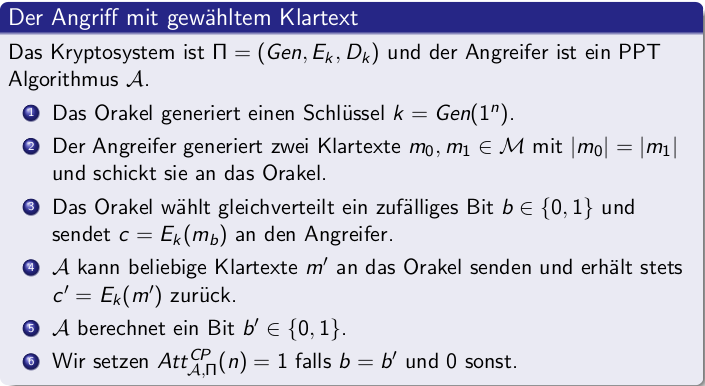
\includegraphics[width = 0.8\textwidth]{CPA1}
\\
$\triangleright $ 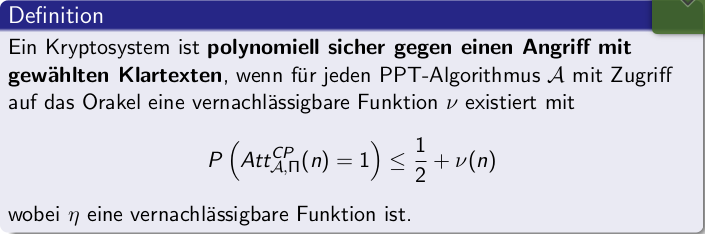
\includegraphics[width = 0.8\textwidth]{CPA2}
\end{document}
